Let
\begin{align}
\vec{A} = \myvec{2 \\ 3 \\ -4} , \Vec{B} = \myvec{1 \\ -2 \\3} , \Vec{C} = \myvec{3 \\ 8 \\ -11}
\end{align}
Then
\begin{align}
\vec{B-A}= \myvec{-1\\-5\\7},
\vec{C-A}=\myvec{1\\5\\-7}
\end{align}
and 
\begin{align}
\vec{M} &= \vec{\myvec{B-A  & C-A}}^T
\\
 &= \myvec{-1 & -5 & 7\\1 & 5 & -7} 
\xleftrightarrow {R_1\rightarrow -R_1}\myvec{1 & 5 & -7 \\1 & 5 & -7}
\end{align}
\begin{align}
\xleftrightarrow{R_2\rightarrow R_2-R_1}\myvec{1 & 5 & -7 \\0 & 0 & 0}
\end{align}
\begin{align}
\implies \text{rank} \myvec{M} &=1
\end{align}
Thus, the points are collinear as can be verified in Fig. \ref{vec/2/24fig: collinear}.
\begin{figure}[!ht]
\centering
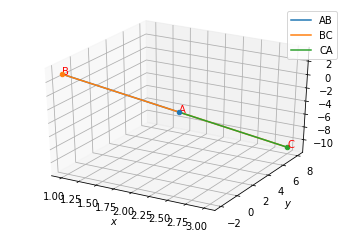
\includegraphics[width=\columnwidth]{solutions/su2021/2/24/figure.png}
\caption{collinear}
\label{vec/2/24fig: collinear}	
\end{figure}
